\documentclass{article}


\usepackage{arxiv}

\usepackage[utf8]{inputenc} % allow utf-8 input
\usepackage[T1]{fontenc}    % use 8-bit T1 fonts
\usepackage{hyperref}       % hyperlinks
\usepackage{url}            % simple URL typesetting
\usepackage{booktabs}       % professional-quality tables
\usepackage{amsfonts}       % blackboard math symbols
\usepackage{nicefrac}       % compact symbols for 1/2, etc.
\usepackage{microtype}      % microtypography
\usepackage{lipsum}
\usepackage{graphicx}
\usepackage{physics}
\graphicspath{ {./images/} }


\title{Event Classification for Higgs Particle with Quantum Machine Learning in 
      High-Energy Physics}


\author{
 Shiwen An \\
  School of High Energy Accelerator Science\\
  The Graduate University for Advanced Studies, SOKENDAI\\
  Tsukuba, Japan \\
  \texttt{shiwenan@post.kek.jp} \\
  %% examples of more authors
   \And
  Xuanqiang Zhao \\
  Department of Computer Science\\
  University of Hong Kong\\
  HK \\
  \texttt{Xuanqiang.Zhao@hku.edu} \\
  %% \AND
  %% Coauthor \\
  %% Affiliation \\
  %% Address \\
  %% \texttt{email} \\
  %% \And
  %% Coauthor \\
  %% Affiliation \\
  %% Address \\
  %% \texttt{email} \\
  %% \And
  %% Coauthor \\
  %% Affiliation \\
  %% Address \\
  %% \texttt{email} \\
}

\begin{document}
\maketitle
\begin{abstract}
Machine Learning Algorithms like Deep Neural Network (DNN), Binary Decision Tree (BDT), has been used in 
high energy physics for a long time, specifically in track signal identification and supervised classification tasks. 
Meanwhile, quantum computing was proposed by Richard Feynman in the early 1980s as a way to performs computations that 
would be unreachable by classical computers. Over the past 40 years, the noisy intermediate-scale quantum computing 
devices have been developed and multiple new algorithms are proposed with such device. In this paper, we present the 
studies of quantum algorithms exploiting machine learning to classify the events of interest from background.
\end{abstract}


% keywords can be removed
\keywords{ Quantum Machine Learning \and Variational Quantum Circuit \and Variational Shadow Quantum Learning \and Quantum Kernel Method\and }


\section{Introduction}
In High-Energy Physics experiments, particles created by collisions are observed by layers of high precision detectors.
In this field, many early attempts to use quantum computing for HEP exist. For example, the data analysis \cite{qml_task1}, identification
of charged particles[], reconstruction of particles collision points []. ([] indicates adding citation based on those paper) As discussed in 
many literatures, the quantum machine learning (QML) is considered as one of the QC algorithms that could bring quantum 
advantages over classical methods[\cite{qml_icepp}, 16].

\section{Task description and data construction}
Discrimination of events of interests is always the most frequently used ML techniques in HEP data analysis. 
In this research, we examine the most frequently used variational quantum classider (VQC), Quantum Kernel Methods, 
Variational Shadow Quantum Learning (VSQL) \cite{qml_vsql} and Quantum Generative Adversarial Network (Quantum GAN). 
\label{sec:headings}
\paragraph{Dataset} Here we use the dataset from UCI's Machine Learning Repository [\href{https://archive.ics.uci.edu/ml/datasets/HIGGS}{Lib}]. 
\paragraph{Task modeling.}
We approach this task as a regression problem. For every item and shop pair, we need to predict its next month sales(a number).
\paragraph{Construct train and test data.}
The dataset provided has 28 features, 21 low-level features and 7 high-level features. 

\subsection{Method 1: Variational Quantum Classifier}

\subsection{Method 2: Variational Shadow Quantum Learning}

\subsection(Method 3: Variational Shadow Quantum Learning)
\lipsum[6]

\paragraph{Paragraph}
\lipsum[7]

\section{Examples of citations, figures, tables, references}
\label{sec:others}
\lipsum[8] \cite{kour2014real,kour2014fast} and see \cite{hadash2018estimate}.

The documentation for \verb+natbib+ may be found at
\begin{center}
  \url{http://mirrors.ctan.org/macros/latex/contrib/natbib/natnotes.pdf}
\end{center}
Of note is the command \verb+\citet+, which produces citations
appropriate for use in inline text.  For example,
\begin{verbatim}
   \citet{hasselmo} investigated\dots
\end{verbatim}
produces
\begin{quote}
  Hasselmo, et al.\ (1995) investigated\dots
\end{quote}

\begin{center}
  \url{https://www.ctan.org/pkg/booktabs}
\end{center}


\subsection{Figures}
\lipsum[10] 
See Figure \ref{fig:fig1}. Here is how you add footnotes. \footnote{Sample of the first footnote.}
\lipsum[11] 

\begin{figure}
  \centering
  \fbox{\rule[-.5cm]{4cm}{4cm} \rule[-.5cm]{4cm}{0cm}}
  \caption{Sample figure caption.}
  \label{fig:fig1}
\end{figure}

\begin{figure} % picture
    \centering
    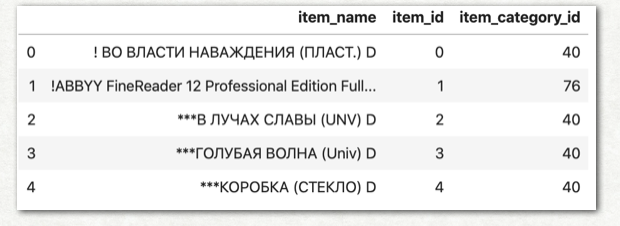
\includegraphics{test.png}
\end{figure}

\subsection{Tables}
\lipsum[12]
See awesome Table~\ref{tab:table}.

\begin{table}
 \caption{Sample table title}
  \centering
  \begin{tabular}{lll}
    \toprule
    \multicolumn{2}{c}{Part}                   \\
    \cmidrule(r){1-2}
    Name     & Description     & Size ($\mu$m) \\
    \midrule
    Dendrite & Input terminal  & $\sim$100     \\
    Axon     & Output terminal & $\sim$10      \\
    Soma     & Cell body       & up to $10^6$  \\
    \bottomrule
  \end{tabular}
  \label{tab:table}
\end{table}

\subsection{Lists}
\begin{itemize}
\item Lorem ipsum dolor sit amet
\item consectetur adipiscing elit. 
\item Aliquam dignissim blandit est, in dictum tortor gravida eget. In ac rutrum magna.
\end{itemize}

\section{Application for Tokyo Institute of Technology}
In the format easier to read before formal submission.
\subsection{Your research topic in Japan: 
Describe articulately the research you wish 
to carry out in Japan.}

Therefore, firstly based on the 
existing “Kernel Regression Imputation in 
Manifolds Via Bi-Linear Modeling: The Dynamic-MRI Case”, 
I do find the proposed problem in the imputation-by-regression 
Specifically, “KRIM makes explicit use of 
(non-linear) manifold assumptions and geometry”. 
There is an interesting point mentioned in this paper, 
where Manifolds learning build on the hypothesis 
that measured data lie close to a low-dimensional 
manifold embedded in a high dimensional space.  
Since I have some familiarity with implementation 
of geometric approaches. I do believe the enhanced data needs 
to be implemented. 

The length of the program is 5 years in total, therefore,
 I would like to explore the quantum computing algorithms 
 with the Riemann Manifold in the first two years. 
 I would like to improve the data analysis method in 
 Variational Quantum Circuit Learning, Quantum Kernel Method 
 and Variational Quantum Shadow Learning with the advantages 
 in Professor Slavakis' lab on Riemannian manifold. 

To understand the research topic, it is necessary to understand what 
currently professor Slavakis is working on. The model heavily involves 
the Manifolds. The kernel regression imputation in manifolds (KRIM).

One question provided to solve: In collected data, "Holes/gaps" or 
"missing entries" give rise in turn to aliasing and motion blurring 
in the observed images series. -> Non-parametric approaches. 

The other question provided is: "Fast Sequential Clustering in Riemannian 
manifolds for Dynamic and Time-series-Annotated Multilayer Networks". This 
work focus on building a sequential-clustering framework able to address 
a wide variety of clustering tasks in dynamic multilayer (brain) networks 
via the information extracted from their nodal time-series. 
There are procedures working step by step: 
\begin{enumerate}
  \item feature extraction from time-series 
  \item Riemannian Manifolds 
  \item Problem: state clustering, community detection, 
  subnetwork sequence tracking.  
\end{enumerate}

First is the Quantum Kernel Method. 
The Quantum Kernel Method formation of 
Reproducing Kernel Hilbert Space (RKHS) with the 
Fast Sequential Clustering in Riemannian Manifolds. 
Quantum Kernel Method was proposed as Quantum Machine Learning.

I will do the emulation first on the normal computer, after verification.
I hope I could access to D-wave to perform the algorithms on the real quantum
computer.  If everything works perfectly, I consider my idea could be 
realized with improvement. 

\textbf{The Top Down Approach:}
One takes the data and analyze with 
different method. First I would like to work on the normal signal processing field 
to study a bit more on classical theory. It is necessary to have 
a deep understanding of the fundamentals before making great 
progress in any field. 

\subsection{Study program in Japan: 
(Describe in detail and with specifics - particularly 
concerning the ultimate goal(s) of your research in Japan)
}

\textbf{The Bottom Up Approach:}
The goals of my research in Japan are composed step by step. 
I would like to enhance the existing algorithms or 
models for data analysis using Quantum Computing Algorithms 
as described in last question. I hope to follow up and expand the 
research shown in previous section and add two or more approaches to build
up a relatively complete "Framework" for quantum signal processing.

\begin{itemize}
  \item Quantum Machine Learning: The Riemannian Manifold Approach
  \item Quantum Signal Processing: Quantum Computing Encoding Theory Approach
  \item Quantum Signal Processing: Quantum Fourier Transform Approach 
\end{itemize}

The combination of the work could build up solid foundations of 
classical signal processing and quantum computing. 

\textbf{Quantum Signal Processing: Quantum Computing Encoding Theory Approach}\newline
Specifically, based on Daan Camps' Paper on "Explicit Quantum Circuits 
for block encodings of certain sparse matrices" and Issac Chuang's paper
on "Optimal Hamiltonian Simulation by Quantum Signal Processing". I could 
see some revolution or breakthrough gradually happen in the field of Signal
Processing. The later one shows the way to simulate the physical systems with 
the quantum signal processing. 

\textbf{Quantum Signal Processing: Quantum Fourier Transform Approach}\newline
The structure for the development of Quantum Signal Processing starts from 
measurement. The wave break down by using Fourier transform's quantum analog
part, Quantum Fourier Transform (QFT). The Quantum Fourier transform could 
particularlly decompose into a product of simpler unitary matrices. 
With Simple decomposition, the discrete Fourier transform on $2^n$ amplitudes 
can be implemented as a quantum circuit consisting of $O(n^2)$ Hadamard 
gates and controlled phase shift gates. 

Borrowed from Qiskit's notation, the classical discrete Fourier Transforms 
act on vector $x = (x_0, x_1,...,x_n)$ and its mapping to vector $y = (y_0, y_1,...,y_n)$
according to formula:
\begin{equation}
  y_k = \frac{1}{\sqrt{N}} \sum^{N-1}_{j=0} x_j \omega_N^{jk}
\end{equation}
Where $\omega_N^{jk} = e^{2\pi i \frac{jk}{N}}$. The quantum state 
$ \ket{X} = \sum^{N-1}_{j=0} x_j \ket{j} $ and mapped to $ \ket{Y} = \sum^{N-1}_{k=0} y_k \ket{k} $ 
and the map could therefore be expressed as:
\begin{equation}
  \ket{j}  = \frac{1}{\sqrt{N}} \sum^{N-1}_{j=0} \omega_N^{jk} \ket{k}
\end{equation}
Or the unitary matrix: 
\begin{equation}
  U_{QFT}= \frac{1}{\sqrt{N}} \sum^{N-1}_{j=0} \sum^{N-1}_{k=0}  \omega_N^{jk} \ket{k} \bra{j}
\end{equation}
There are already well published paper for quantum Fourier transform. In imaging analysis, 
Fourier transform is definitely an unavoidable technique. Starting from here, 
in analog signal processing, I would like to apply quantum Fourier transform, 
the classical discrete Fourier transform and compare their differences and how 
quantum Fourier transform could possibly enhance the classical result. 
Several Goals for working on Quantum Fourier Transform:
\begin{enumerate}
  \item Forming algorithms could possibly enhance or replace the classical 
  discrete Fourier transform. Such replacement may improve classical 
  algorithms to achieve better performance, like noise filtering and etc. 
  \item By the theory of Big-O, the quantum Fourier transform is exponentially 
  faster than classical discrete Fourier transform. 
\end{enumerate}


The first paper is the more recent one, which introduced the 
more efficient way to encode the data. 

A fundamental method or algorithm in exploring today's 
hard question in natural science. Not only in biomedical science, 
neurological science, fMRI, but also in gravitational 
wave detection, detection of Higgs particles and more. 
Of course, this could not be simply developed with purely 
algorithm solutions, collaboration with other teams and
 more will be necessary. 

The Ultimate goal is to explore the 
 Ubiquitous quantum signal processing or 
 quantum machine learning in natural science and more. 
This is a type of engineering goal which could possibly expand the 
 field of signal processing. 

The PhD
Thesis by Doctor Yonina Eldar and A.V. Oppenheim.

\bibliographystyle{unsrt}  
%\bibliography{references}  %%% Remove comment to use the external .bib file (using bibtex).
%%% and comment out the ``thebibliography'' section.


%%% Comment out this section when you \bibliography{references} is enabled.
\begin{thebibliography}{1}

\bibitem{qml_icepp}

\bibitem{qml_vsql}
Li, G., Song, Z., \& Wang, X. (2021). 
VSQL: Variational Shadow Quantum Learning for Classification. 
Proceedings of the AAAI Conference on Artificial Intelligence, 35(9), 8357-8365. \url{https://doi.org/10.1609/aaai.v35i9.17016}

\bibitem{qml_task1}
Mott, A., Job, J., Vlimant, JR. et al. Solving a Higgs optimization problem with 
quantum annealing for machine learning. Nature 550, 375–379 (2017). \url{https://doi.org/10.1038/nature24047}

\bibitem{kour2014real}
George Kour and Raid Saabne.
\newblock Real-time segmentation of on-line handwritten arabic script.
\newblock In {\em Frontiers in Handwriting Recognition (ICFHR), 2014 14th
  International Conference on}, pages 417--422. IEEE, 2014.

\bibitem{kour2014fast}
George Kour and Raid Saabne.
\newblock Fast classification of handwritten on-line arabic characters.
\newblock In {\em Soft Computing and Pattern Recognition (SoCPaR), 2014 6th
  International Conference of}, pages 312--318. IEEE, 2014.

\bibitem{hadash2018estimate}
Guy Hadash, Einat Kermany, Boaz Carmeli, Ofer Lavi, George Kour, and Alon
  Jacovi.
\newblock Estimate and replace: A novel approach to integrating deep neural
  networks with existing applications.
\newblock {\em arXiv preprint arXiv:1804.09028}, 2018.

\end{thebibliography}


\end{document}
